% !TEX root = ../thesis-main.tex

\chapter{Metrics as Losses}
\label{chapter:research-sigmoidf1}

\if0
nth step in personalization pipeline...
motivation...
gap...
how it fits in the thesis
\fi

\begin{figure}[ht]
  \centering
  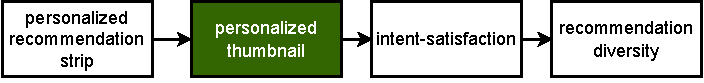
\includegraphics{images/pipeline_step2.pdf}
  \caption{The second step of the personalization pipeline}
  \label{fig:pip2}
\end{figure}

\footnote[]{This chapter was published at the Transactions of Machine Learning Research (TMLR) under the title ``sigmoidF1: A Smooth F1 Score Surrogate Loss for Multilabel Classification'' \citep{sigmoidf1}.}
\acresetall

After a recommendation model outputs video titles in the first step of the personalization pipeline, we still have to represent each video via an image. For that we revisit a classical classification problem. Namely we take videos recommendations generated via a diffusion model and perform multilabel classification on thumbnails of these videos with our custom loss sigmoidF1. By that process, we hope to provide personalized thumbnails of the video for each user. There is little work beyond blog posts on how to personalize thumbnails on recommendation platforms. Under the pretense of handling this in an algorithmic way, we point out the lack of loss functions speficially designed for the multilabel classification problem in general
%We propose to handle this in a systematic way, and propose a first loss function specifically designed for multilabel classification on the entire stochastic gradient descent training batch.
This part of the personalization pipeline is focused on the following question:

\medskip
\noindent
\textbf{\ref{rq:sigmoidf1}:} \acl{rq:sigmoidf1}
\medskip

We tackle this question, by simplifying the problem first. Let's assume each user has a preferred movie genre. Then we would like to serve each user with that preferred genre. Given a set of candidate thumbnails, how can we determine which genre(s) they relate to the most? At inference time, we try to optimize for rather comprehensive metrics like F1: it can balance true positives, false positives and false negatives. At training time, we use classical multilabel classification, but propose our own loss function, sigmoidF1. This loss function is a surrogate of the F1 classification metric. As such we propose a metric as a loss.




\subimport{multilabel/sigmoidF1/sections}{01-introduction}
\subimport{multilabel/sigmoidF1/sections}{02-background}
\subimport{multilabel/sigmoidF1/sections}{06-related-work}
\subimport{multilabel/sigmoidF1/sections}{03-method}
\subimport{multilabel/sigmoidF1/sections}{04-experimental-setup}
\subimport{multilabel/sigmoidF1/sections}{05-experimental-results}
\subimport{multilabel/sigmoidF1/sections}{07-discussion}
\subimport{multilabel/sigmoidF1/sections}{08-conclusions}

\section{Upshots for the personalization pipeline}

\if0
in this chapter, ...
how we answered the research question
future work

in the next chapter we continue...
2 sentences
\fi

In this chapter we constructed a surrogate to the F1 metric, that is differentiable everywhere at training time.  Thanks to that loss function, we are able to train image models that categorize thumbnails into an optimal set of categories (as defined by the F1 score). But this endeavor is only a small step towards two separate avenues.
\begin{enumerate*}[label={(\roman*)}]
\item If our goal is to optimize for certain non-differentiable metrics at inference-time, why don't we use more metric surrogates as losses at training-time?
\item In the future, we could think of generating thumbnails or movie posters from scratch for each user, based on their preferences.
\end{enumerate*}

In the next chapter, we take a step back. Once we have served personalized recommendations with personalized thumbnails, we look at how the user behaves on the platform over time. More precisely, we combine the observable user behavior data (e.g. clicks) with unobservable intents (e.g. bookmark videos to watch later) to predict the satisfaction of that user.


\section*{Reproducibility}
To facilitate the reproducibility of this work, our code is available at \url{https://github.com/gabriben/metrics-as-losses}.


\begin{appendices}
\chapter{Appendix of Metrics as Losses}
\subimport{multilabel/sigmoidF1/appendix}{appendix}
\end{appendices}



%%% Local Variables:
%%% mode: latex
%%% TeX-master: "../thesis-main"
%%% End:
